\documentclass[a4paper]{article}
\usepackage[utf8]{inputenc}
\usepackage{graphicx}
\usepackage{onecolceurws}
\usepackage{xcolor}
\usepackage{url}

\def\infinity{\rotatebox{90}{8}}

\title{DameGender: Towards an international and free dataset about name, gender and frequency}

\author{
David Arroyo Menéndez, Madrid, Spain \\ \{davidam@gmail\}.com
}

\newif\ifdraft
\drafttrue
%\draftfalse
\input{macros}

\institution{DAMEGENDER}

\begin{document}

\maketitle

\begin{abstract}
  %% Introduction

  Equality of gender is the fifth objective of sustainable development
  for United
  Nations\footnote{https://www.un.org/sustainabledevelopment/gender-equality/}.

  This equality can be reached by measuring and analyzing data
  and making good politics with the results. Many gender studies
  count males and females based on their names, for
  instance, research papers, job positions, streets, etc. The
  traditional research method is to use commercial APIs with
  proprietary data without idea about how the data was collected.
  Data may also be gathered from Wikipedia, lingüistic studies,
  scientific sites, or statistical offices.

  %% Methodology

  This approach is based collecting Open Datasets regarding name,
  gender and frequency from many statistical institutions. So, we
  need a scientific discussion about unifying formats and processing
  data easily.

  Therefore, Damegender (Free and Open Source Software) to retrieve
  and make calculus with these data.

  %% Results

  The dataset we used covers more than 20 countries in the occidental
  world encompassing many names with an accuracy of approximately 90%
  with it. This will create to measure gender gap to students and
  academics interested on the phenomenon without costs and on a
  reproducible way and more people will be contributing to fix the
  gender gap.

  %% Conclusion

  Free software and the data provided by statistical institutions make
  it possible to produce reproducible research for peer review. Thus,
  semantics and diversity can be more easily addressed.
  
\end{abstract}

\section{Introduction}
The United Nations has a goal to address the gender
gap\footnote{https://www.un.org/sustainabledevelopment/gender-equality/},
but ``if you cannot measure it, you cannot improve it"~\cite{thompson1833electrical}
and ``Software Engineering Economics is an invaluable guide to determining
software costs, applying the fundamental concepts of microeconomics
to software engineering~\cite{barry1981software}''. Free software and open
data lead to a reduction in costs, for example, many people and
institutions is using LibreOffice and Ubuntu (GNU/Linux) to avoid paying
the fees with similar products such as Microsoft Windows and Microsoft
Office. Gender detection tools based on the user name is based on API
solutions, providing a free software and open data solution. This will
createit competition in a market without a very strong leader, avoiding
payments and strategizing profits from a trademark, such as, Firefox or
Chrome.

Through the use of personal names, one may infer gender on
academical papers, books, newspapers and many interactions on Internet.
So, detecting gender from the names may be a strategical way to
measure gender gap.

Many users today are using APIs such as Genderapi, Genderize,
Namsor, or NameApi, Wikipedia, or Free Software solutions
(NLTK\cite{loper2002nltk}, R Gender, Gender Detector and Gender
Computer\footnote{https://github.com/tue-mdse/genderComputer}.

Traditional open source solutions has a few number of names due to
use files of a single country or being software not maintained in
the long time. And Wikipedia is storing few names per country.

However, the gender gap is a problem recognised in United Nations and
the IT market is leading big inequalities in economic and gender gap.
This article presents data collected to assist in finding the solution
to a number of problems (search engine, infering gender in csv files,
names in different countries, wide dataset) faced by
the industry as well as other problems not solved in an industrial way
such as counting males and females in GitHub repositories, mailing lists,
etc.

A previous study~\cite{karimi2016inferring} dicussed these datasets as
a way to improve their accuracy, comparing tools that use different
public datasets (SSA~\footnote{https://www.ssa.gov/oact/babynames/limits.html},
IPUMS~\footnote{https://usa.ipums.org/usa-action/variables/NAMEFRST},
namdict~\footnote{https://raw.githubusercontent.com/lead-ratings/gender-guesser/master/gender\_guesser/data/nam\_dict.txt}, etc)

So, a goal is to augment the number of names using official statistics
and taking into account diversity goals such as non binary gender and
cultural minorities.

With DameGender we will make science reproducible\cite{peng2011reproducible}
in fields with similar works such as Natural Language Processing
(gender detection from the name~\cite{sun2019mitigating}), social
sciences or journalism (gender
gap~\cite{holman2018gender,mislove2011understanding,niemi2017gendered,de2014genero}),
linguistic~\cite{hutson2016gender,al2009socio},
software engineering~\cite{vasilescu2012gender}, among other fields.

The remainder of this article is structured as follows:

Section~\ref{sec:stateofart} presents the main research measuring the
gender gap and gender detection tools using name.

Section~\ref{sec:design} gives vocabulary and philosophy about to
choose sources and to face the diversity troubles building a dataset.

Section ~\ref{sec:measuring} explains an application for this
dataset: to measure gender gap in GNU/Linux.

Section~\ref{sec:conclusions} points a summary about this approach and
future works.

The contributions of this article are:

1. An integrated solution in the different applications field relative
to inferring gender from the name.

2. A collection of open datasets retrieved from statistical sources
and standardized in an unique format.

3. A new study applying DameGender to count males and females in
GNU/Linux.

4. An approach based on reproducible results.

Many articles related are about to apply machine learning techniques,
but using only Open Data is possible to acquire very good accuracies.
So, this work is augmenting the base of truth of the state of art
related to Open Data, so this work is helping to look for datasets
checking accuracies with several data sources in statistical
institutions and other Open Data trust sources as Wikipedia,
Project Gutenberg, Amazon, sport institutions, Forbes, etc.

\begin{figure}
  \centering
  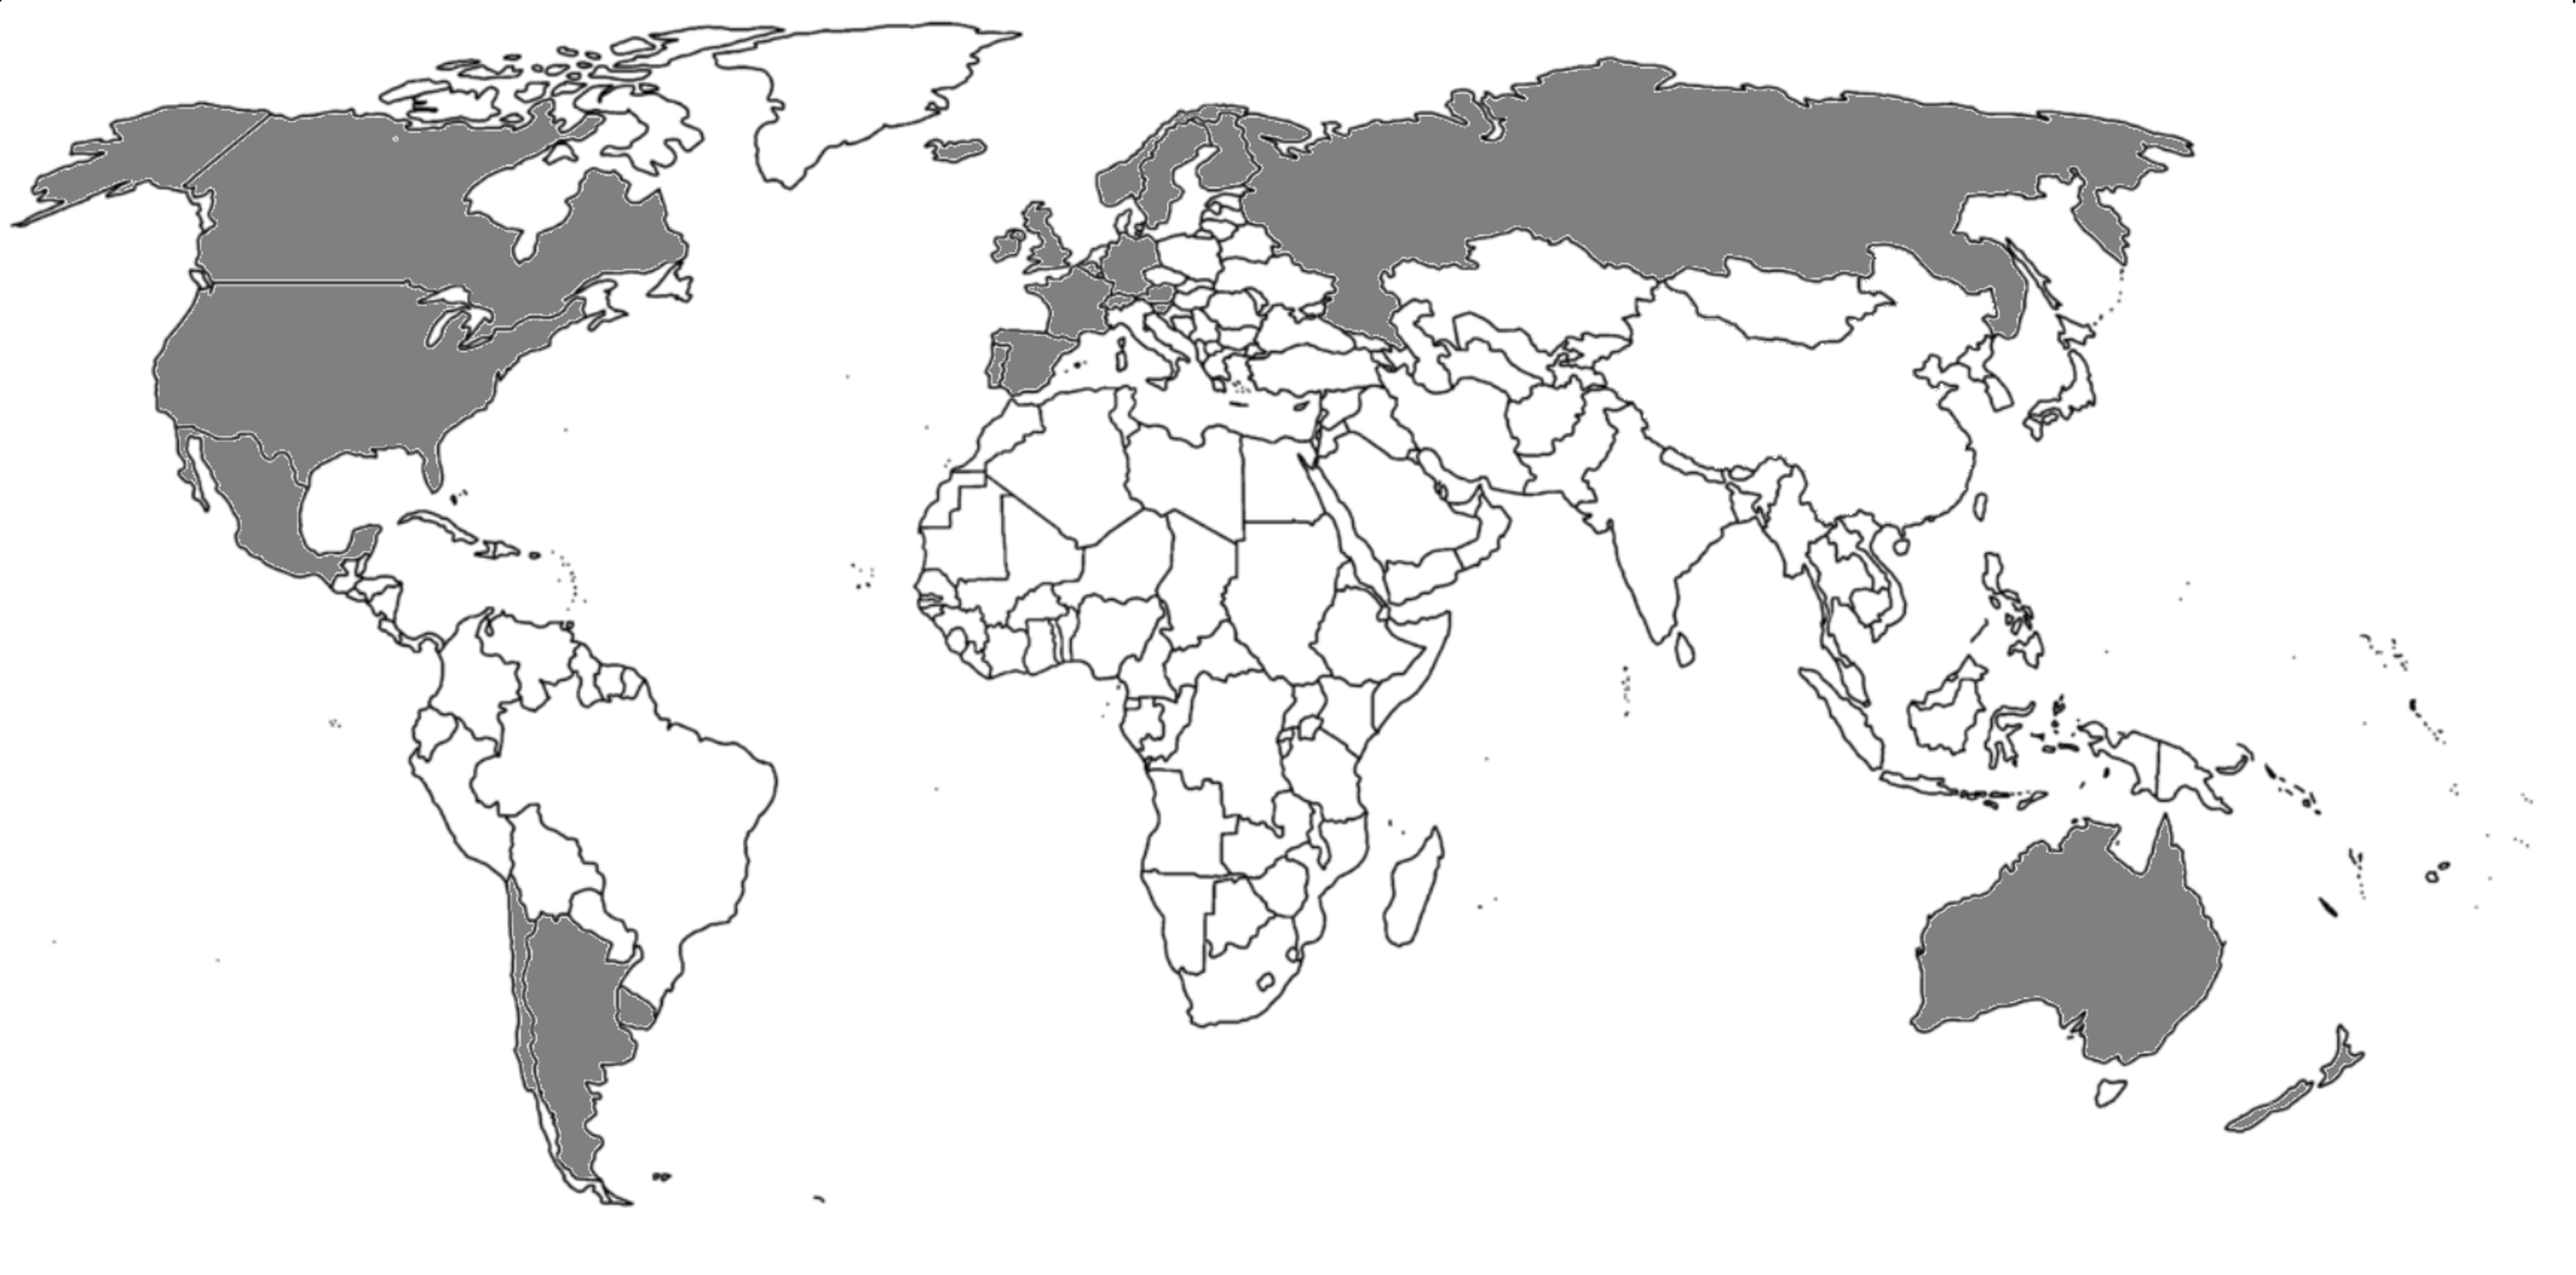
\includegraphics[width=0.6\textwidth]{images/mapamundi-politico-mudo.pdf}
  \caption[Caption for LOF]{Grey (Countries with Open Data provided by Statistical Institutions), White (Countries without Open Data or don't reproduced by the author)}
\end{figure}

\section{State of the Art}
\label{sec:stateofart}

\subsection{About Gender Gap}

To reduce gender gap refers to equality between males and females,
and non discrimination policies. Gender refers to the sex of a person
determined in the moment of the birth, although it can be changed
throughout life. Discussions about gender definitions refers to these
problems. However, there is a consensus determining gender, frequency
and names with official statistics released by the institutions in the
states.

Measuring the gender gap requires set indicators. Global Gender Gap
Report~\cite{chancel2022world} has been proposed economy, health,
education and politics. The United Nations
site\footnote{https://www.unwomen.org/} is showing indicators
to measure disparities such as laws, education, maternal mortality,
political participation, poverty, domestic work, gender parity in
the work, to access to the economy, youth issues (access to
studies and/or work), violence against women, climate justice,
access to the justice, health, etc.

It's possible to make impactful decisions on an issue through research
results that have taken these indicators into consideration. For example,
Miyake and other authors ~\cite{miyake2010reducing} concluded that making
affirmations about ethical values reduced the gender achievement gap in colleges.

Related to measuring the gender gap in social research,
Bimber~\cite{bimber2000measuring} presented two factors affecting
the gender gap on the Internet (access and use) by socioeconomic and gender
reasons in a survey that collect data over several years.

\subsection{Counting males and females on the Internet. Why? Where?}

This work focused on retrieving data from secondary sources such as
GitHub, Wikipedia, APIs, websites in general, mailing lists, etc.
Previous research works about factors modifying several gender gap
indicators (economy, education, politics) were obtained from secondary
sources.

For example, a social scientist studying gender gap in
journalism~\cite{alvarez2012journalism} can count males and
females on Twitter. These metrics are important because the journalism
is evaluating gender gap in political, education, or the economy,
etc. Meanwhile, Computer Science making research about how to
count males and females in Twitter~\cite{burger2011discriminating}. In
these studies the name, nickname, photo, and identifying gender are
retrieved from these data.

Burger and others~\cite{burger2011discriminating} presented
several configurations of a
language-independent classifier for predicting the gender of Twitter
users. The large dataset used for the construction and evaluation of
these classifiers was drawn from Twitter users who also completed blog
profile pages.

Understanding the demographics of twitter users~\cite{mislove2011understanding}
analyzed the Twitter population, including the gender. The gender
was inferred making queries from the names to the dataset provided
by the United States Census Bureau.

Wagner and others~\cite{wagner2015s} analyzed the gender gap in Wikipedia,
showing evidence of more subtle forms of gender inequality explaining
how to solve these evidences. To measure gender inequality has been
developed the next bias: coverage, structural, lexical (ex:
discriminatory words for women), and visibility.

Computer Science is generating many Forbes billionaires and the public
code may help to understand the gender gap in this field, which may
have some importance to the economy. Public repositories can
be used to build indicators about the economy in Computer Science with
more factors, such as job positions, value of companies, etc.
Arjona and others~\cite{10.1007/978-3-319-39225-7_13} published in 2016
a survey of 2000 contributors where showed that the female participation would be
around 2\% to 5\%. Izquierdo and others~\cite{izquierdo2018openstack}
revealed that few females contribute code or take political
responsability in the OpenStack community.
Recently, Zacchiroli~\cite{zacchiroli2020gender} conducted the first large-scale
longitudinal study of gender imbalance among authors of
collaboratively developed, publicly available code, where
contributions by female authors remain scarce less that 8 \% of
commits was able to be detected were from women, confirming decades of
gender imbalance in Free/Open Source Software (FOSS). Steffano used
to namdict~\footnote{https://raw.githubusercontent.com/lead-ratings/gender-guesser/master/gender\_guesser/data/nam\_dict.txt} dataset with genderguesser to infer gender from
the name. Vasilescu and others~\cite{vasilescu2015gender} determined
that women programmers are in the minority in OSS and other technical
fields, although increased gender and tenure diversity is associated
with greater productivity. Vasilescu and others~\cite{vasilescu2012gender}
explored the popular Q\&A about technological issues called
StackOverflow, which summarizes that the percentage of women engaged
in SO is greatly imbalanced, and men represent the vast majority of
contributors.

Related to the gender gap in science, Cassidy R. Sugimoto and
colleagues~\cite{lariviere2013bibliometrics}
present a very good bibliometric analysis confirming that gender
imbalances persist in research output worldwide. Holman and
others~\cite{holman2018gender} presented a code in R
using genderize API and providing a good approach
about how to calculate gender gap inferring gender from an author
names retrieved from arXiv. 

\subsection{Automatic approaches to infer gender}

There are several ways to infer gender from Internet
sources: hand written, images, documents and names.

Liwicki and others~\cite{liwicki2011automatic} presented a method
inferring gender from hand written texts with a 67.5 \% accuracy.

Gallagher and others~\cite{gallagher2008estimating} combines
image based gender and age classifiers with the cultural 
information provided by first names to recognize people
with no labeled examples with results near to 60 \% accurate.

Argamon and others~\cite{argamon2003gender} explains that
females use many more pronouns, while males use many more
noun specifiers, in a large subset of the British National
Corpus covering a range of genres. Therefore,
Koppel and others~\cite{koppel2002automatically} presented
a document classification system with accuracy of
approximately 80 \%. Cheng and others ~\cite{cheng2011author}
exposes a feature selection and a model built using machine learning
resulting in 85.1 \% accurate rate for identifying gender from text.

\subsection{Infering gender from name}

The tools used to infer gender from a name are tipically based on
datasets that, at a minimum, is include gender and name as minimum.

Liu and others~\cite{liu2013s} presented a method to infer gender
from first names in Twitter, the dataset was hand coded by agreement
between three Amazon workers with 50,000 Twitter users select at
random with only 12,681 gender labels. The goal of this study was
to determine the incremental value of using the user name as a feature
in gender inference based on tweets.

Mueller and others~\cite{mueller2016gender} presented how to
infer gender in Twitter. They used namdict and the United States
census as datasets. The features were 'number of consonants',
'number of vowels', 'number of syllables', 'number of bouba
consonants', 'number of bouba vowels', 'number of kiki consonants',
'number of kiki vowels'. The classification model was created using SVM.

\subsection{Related ideas}

Ambekar and others~\cite{ambekar2009name} presented a
system to classify name and ethnicity from open sources
using machine learning to extract a name list from Wikipedia.
A more recent work is guided by Rodríguez
Pérez and others~\cite{nadri2021relationship}, in
which presented NamPrism giving fresh ideas classifying
races and being applied to massive software repositories.

Bollegala and others~\cite{bollegala2010automatic} presented
another approach that
used a lexical-pattern-based approach to extract aliases of a
given name, with a set of names and their aliases as training
data to extract lexical patterns. The candidates are ranked
using various ranking scores. Support vector machines were
used to construct the ranking function.

\subsection{Related Standards}

ISO/IEC 5218 proposes the following norm about coding
gender: ``0 as not know'', ``1 as male'', ``2 as female''
and ``9 as not applicable''.

The RFC 6350
(vCard)~\footnote{https://datatracker.ietf.org/doc/html/rfc6350}
has these categories: ``m as male'', ``f as
female'', ``o as other'', ``n as not applicable'' and ``u as
undefined''. Based on this standard, those conducting web
publishing can use CSS classes using a web standard such as
h-card~\footnote{https://github.com/microformats/h-card}
microformats in the context of to write forms in web interfaces
consider w3 lectures~\footnote{https://www.w3.org/International/questions/qa-personal-names}

\subsection{Summary}

The first name of a subject is the is the key factor used to
determine gender in the State of Art gender inference tool.
However, in many contexts there are more features: surnames,
text, images, nicknames, etc. The first name can be useful to
infer another stuff such as race, ethnicity or culture, too.

Machine learning and the previous features selection is being
used in many works, although there is an open discussing as
to which is the best approach

The datasets can be built by human experts, although there are
some open datasets used several times in these researches, such as
namdict, or the United States census.

\section{Design}
\label{sec:design}

\subsection{Truth and falsehood in names, gender, and frequency}
\label{sec:truthandfalsehood}

The current idea in the field accepts that using name, gender and
frequency is ok because there are people paying for or downloading
a product. Typically, this is an acceptable assumption, although
the consumer may purchase a bad product due to a good marketing
strategy, a monopoly or there is a fraud, etc. Consumers may also 
trust in the government statistics regarding the economy,
demography, or democracy. Therefor the people may trust the data
for names, gender, and frequency. The
Damegender\footnote{https://damegender.davidam.com} point of view
is to trust in: the market tools and the official statistics.

Sometimes there are problems downloading official statistics, but
there are people who have retrieved these data with web scraping.
These files with another idea about truth.

Another problem arises when the government changes the data,
sometimes communicating it to the users and other times
not. This may be problematic for upgrades, but not with the truth,
since changes can be traced. 

With an international free dataset of names, gender, and frequency,
we can build reproducible science in fields such as natural language
processing (gender detection from the name), the social sciences, 
journalism (gender
gap~\cite{holman2018gender,mislove2011understanding,niemi2017gendered,de2014genero}),
linguistics~\cite{lawson2005russian,krueger1962mongolian,van2020gender,agyekum2006sociolinguistic,fraser1987lexicon},
or software engineering~\cite{vasilescu2012gender}.

\subsection{Gender, language, nation and diversity}
\label{sec:diversity}

There are rules and exceptions in different languages to predict if
a name is about male or female. For example, in Spanish or English,
there are more names ending with 'a' classified as females than
classified as males. However, Andrea is female in Spain and
male in Italy. So, it is useful to understand the language and culture
associated with a name. Language is close to nation, but there are
differences, for example, in Spain there are several languages Basque,
Catalan, Castillian. Spanish is the main language in Spain.
and in other countries such as Argentina, Mexico, Ecuador and Bolivia,
Thus, it is helpful to know the language and nation a name or surname
has originated from to help to detect gender.

Some countries, such as Spain, are providing free datasets for
surnames but we need more efforts from many countries on this
objective. However, Wikipedia and machine learning are working
to relate names and surnames with ethnicity~\cite{ambekar2009name}.

\subsection{Damegender open datasets collection}
\label{sec:damegender}

Damegender\footnote{https://github.com/davidam/damegender}
unified the different formats for name, gender,
and frequency from statistical offices of the following countries:
Argentina, Austria, Australia, Belgium, Canada, Switzerland, Germany,
Denmark, Spain, Finland, France, Great Britain, Ireland, Iceland,
Norway, New Zealand, Mexico, Portugal, Russia, Slovenia, Sweden,
the United States of America and Uruguay. There are datasets as Italy,
Brazil or China that has been found scraped from statistical institutions,
we are evaluating the quality of these datasets and will be included
in the future if it possible demonstrate the quality of these datasets.

Is has been developed several python commands to collect datasets,
but the good idea is to make a single command unifying all efforts.
Now it is called orig2.py and it calls a single sh script per country
with statistical office using open data for names, gender and frequency
and makes the preprocessing. The test datasets, wikidata sources
and API sources must be unified with orig2.py in a
single command, with a single interface, perhaps inspired in apt
(debian command), or pip (python command).

It has been applied the criteria that one person usign a name is
a gender vote (male or female)\footnote{On the future, laws about
non binary could be including other options, but only male and
female was found as valid options in the open datasets when this
article is being written}. So, for each country has been choosen
births or total of people using names in the country. Later, it
has been merged these datasets building a free and international
dataset. 

Damegender uses surnames given by statistical institutions (Spain,
Russia, the United States of America and Argentina in this moment).
However, there are few statistical institutions that provide
surnames and the lingüistic diversity is a good point, has been
added surnames for all countries from Wikidata. Perhaps in the future
Wikidata will become the best source of data for names and surnames,
but now there are few elements.

When the work is finished, we could to rebuild machine learning models
to predict new names and nicknames in any language and culture. The
results is the longest list of public names with a scientific approach.

\begin{table}[t]
\footnotesize
\begin{tabular}[]{lcccc}
  \hline
  Dataset & SSA & namdict & NLTK & Damegender \tabularnewline
  males & 91.320 & 48.821 & 2.943 & 257.925 \tabularnewline
  females & 91.320 & 48.821 & 5.001 & 304.553 \tabularnewline
  \hline
\end{tabular}
\caption{Comparison of the number of names between open data solutions}
\label{table:DifferentNamesMeasures}
\end{table}

A possible criticism about this approach is the Leslie
Problem\cite{blevins2015jane}: the match between gender and name
depends of the year. The solution to this problem is to introduce the
age of the person in question. The most common use case states that
the input is the name and the output must be gender, frequency and
percentage. Therefore, a decision about gender must be made without
data on the age or surname in most cases. This dataset was designed for
the most of used use cases. We can take into account other inputs,
such as surname or age to improve the accuracy. There are many open
datasets with names and frequencies that have been classified by years.
Therefore, this problem can be fixed with open data, too.

\begin{table}[t]
\footnotesize
\begin{tabular}[]{lcccc}
  \hline
  Dataset  & Accuracy & Precision & Recall & F1-Score  \tabularnewline
  Damegender &  0.8756  & 0.9638    & 1.0    & 0.925  \tabularnewline
  \hline
\end{tabular}
\caption{Several precision measures about the DameGender international dataset}
\label{table:DifferentAccuracyMeasures}
\end{table}

We have measured about the international DameGender dataset,
using the dataset test made by Santamaria and Mihaljevic
\cite{10.7717/peerj-cs.156} reaching: accuracy (0.8756), precision
(0.9638), recall (1.0) and f1-score (0.925). With other test datasets,
similar and better results:

\begin{table}[t]
  \footnotesize
  \begin{tabular}[]{lc}
    \hline
    Dataset & Accuracy  \tabularnewline
    Scientists Wikipedia & 0.93 \tabularnewline
    FIFA soccer & 0.93 \tabularnewline
    WTA tenis & 0.91 \tabularnewline
    National League & 0.91 \tabularnewline
    Baby Names New York & 0.98 \tabularnewline    
    Conseil Garonne & 0.97 \tabularnewline
    P Sebo\cite{sebo2021performance} & 0.88 \tabularnewline
    Santamaria \& Mihaljevic\cite{10.7717/peerj-cs.156} & 0.88 \tabularnewline
  \end{tabular}
  \caption{Accuracies using several test datasets about the DameGender international dataset}
  \label{table:SeveralTests}
\end{table}

\subsection{Free APIs for free datasets?}
\label{sec:freeapis}

There area number of open data websites that allow the user to retrieve structured open data without cost. These sites include Wikipedia with SPARQL and OpenStreetMap with API rest, among others.

The open datasets for names, gender, and frequency are being modified once a year, at most for each statistical institution.

DameGender contains python scripts designed to create the
different datasets and publish json files that could be used as a free
API rest publishing the json files in sites as GitHub pages, GitLab
pages, or similar sites with free uploads.

\begin{verbatim}
  $ cat DAVID_all.json
  [{
      "name": "DAVID",
      "frequency": 4856689,
      "males": "99.73267796229078 %",
      "females": "0.26732203770922947 %"
  }]
\end{verbatim}

Therefore, it may be possible to have free API rest about names,
gender, and frequency with reduced costs to fix the gender gap
in a collaborative way similar to Wikipedia, OpenStreetMap or
many free software projects.

\section{Measuring gender gap. GNU/Linux as use case}
\label{sec:measuring}

With a trust open dataset for names, gender, and frequency it is
easy to measure the gender gap. Students and academics could
measure the gender gap inexpensively and meet the fifth
Sustainable Development Objective of the United Nations,
which is to erase the gender gap completely. 

This section is divided into counting males and females using
Debian, GNU, and Linux.

It has been obtained the csv files using different methods
to determine the names about the people in these communities.

In the Debian community all members must collaborate with
a gpg key, so we can count males and females from the keyring.
The keyring was imported with gpg commands and later 
the keyring was placed in a csv file.

GNU\footnote{https://www.gnu.org/people/} and
Linux\footnote{https://www.kernel.org/doc/html/latest/process/maintainers}
have collaborative websites for these projects. Therefore, making web
scraping scripts has been downloaded the people and processed
the people to csv files in this experiment.

In DameGender, has been developed csv2gender, a software with a csv
file as input and deployed a statistics graph and/or return the result
of males, females and unknowns about the input.

To make easy to reproduce the experiment we are pasting the commands
used with a modern version of Damegender.

\begin{verbatim}
python3 csv2gender.py files/gnu.csv
 --first_name_position=0
 --title="GNU maintainers grouped by gender"
 --dataset="inter"
 --outcsv="files/gnu.gender.csv"
 --outimg="files/gnu.gender.png"

python3 csv2gender.py files/linux.csv
 --first_name_position=0
 --title="Linux maintaners grouped by gender"
 --dataset="inter"
 --outcsv="files/linux.gender.csv"
 --outimg="files/linux.gender.png"
 --delete_duplicated

python3 csv2gender.py files/debian.csv
 --first_name_position=0
 --title="Debian maintaners grouped by gender"
 --dataset="inter"
 --outcsv="files/debian.gender.csv"
 --outimg="files/debian.gender.png"
 --delete_duplicated
\end{verbatim}

\begin{figure}
  \centering
  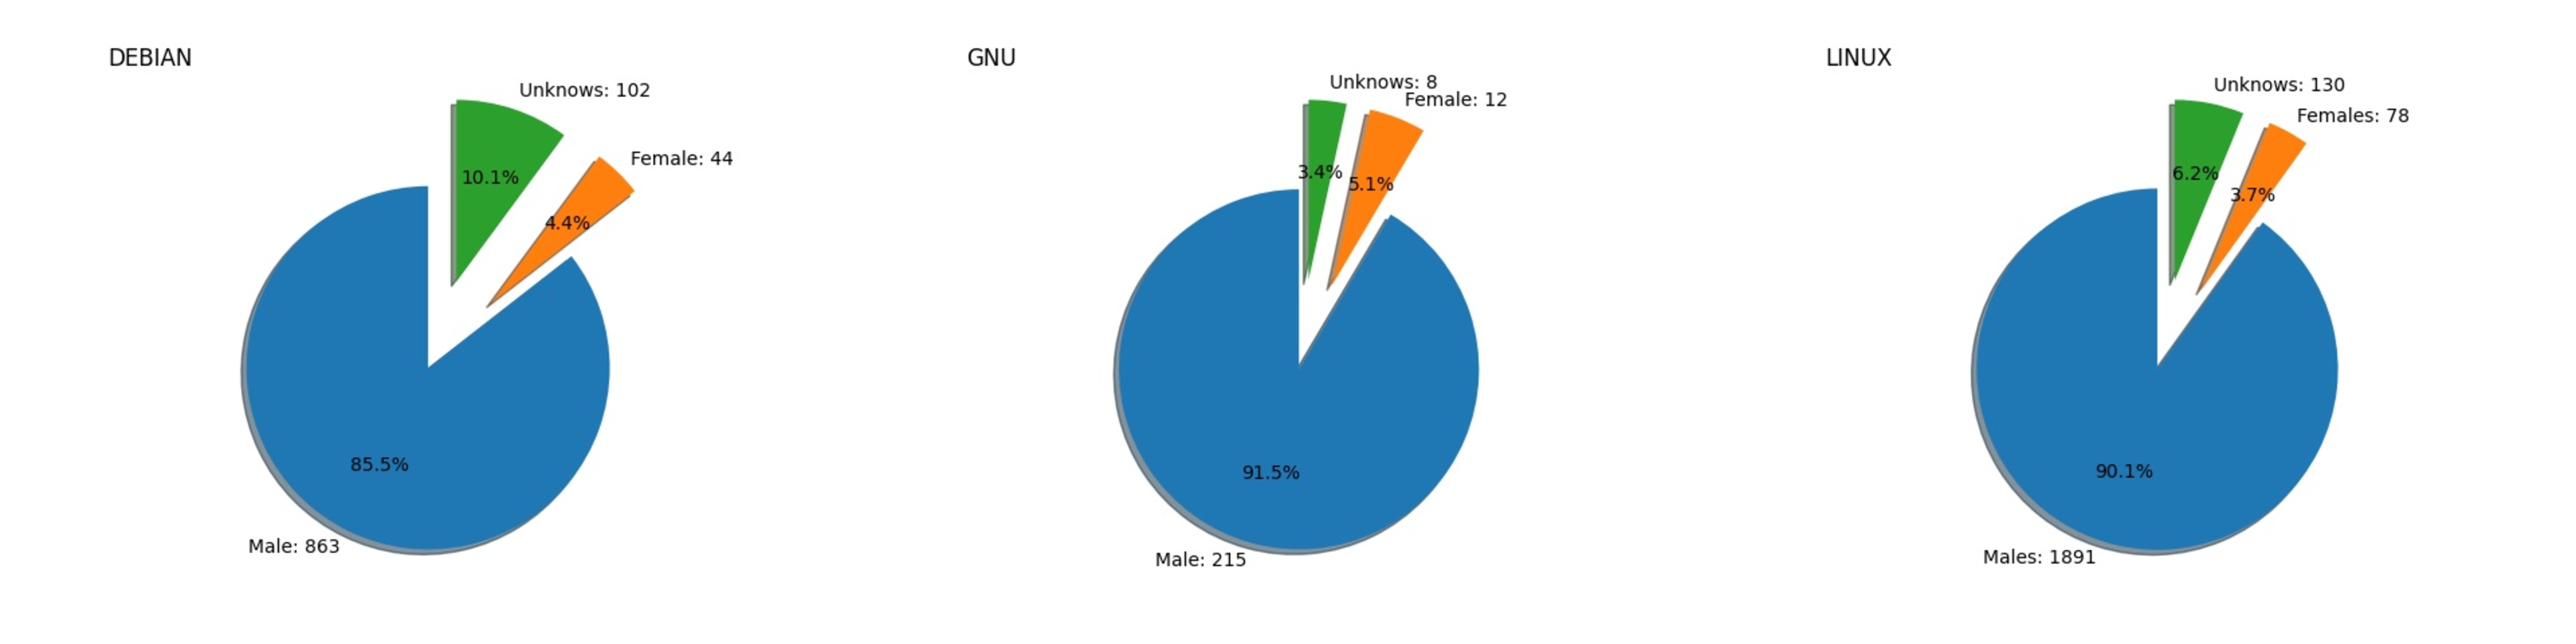
\includegraphics[width=0.6\textwidth]{images/debian_gnu_linux.pdf}
  \caption[Caption for LOF]{Males (blue), Females (orange) and Unknows (green) in Debian, GNU and Linux}
\end{figure}

The inter dataset was created by merging several open datasets
downloaded from official statistics sites from different nations,
being a good representation of the Western World and the free
software world is populating this world's area\cite{gonzalez2008geographic}.

Linux divides the developers in 1891 males (90.1\%), 78 females
(3.7\%) and 130 unknowns (6.2\%). The number of unknowns is due to
different reasons, but it's so common in Linux that the developer is a
company and not a name of a person.

GNU divides the developers in 215 males (91.5\%), 12 females (5.1\%)
and 8 unknowns (3.4\%) Richard Stallman, the GNU founder returned to
be president apologizing by his personal behaviour with the
females.\footnote{https://www.fsf.org/news/rms-addresses-the-free-software-community}

Debian is a distribution, the project who makes the CD/DVD and the
software ready to be downloaded from Internet with the
dependencies. There are many distributions, such as, Ubuntu or RedHat
so it is not representative, but it's interesting to understand that
the numbers are similar in Debian dividing the developers in 863 males
(85.5\%), 44 females (4.4\%) and 102 unknowns (10.1\%).

%% \includegraphics[width=0.9\textwidth]{images/debian.gender.pdf}

\section{Conclusions and Future Works}
\label{sec:conclusions}

Data feminism\cite{d2020data} is an area of growing interest.
It has been explained the DameGender application,
the motivations (reproducible research, fix gender gap to solve the
United Nations objective, fields of application, including linguistic,
social sciences, software engineering, natural language processing and
journalism).

An improvement would be to build an international, universal, and free
dataset of names, gender and frequency for the right design with
the current state of the job, attending to the diversity (LGBT
options, cultural minorities, etc.).

This article has explained the technologies involved in reducing costs
related to studying the gender gap about gender gap (gender detection
from the names, API rest, semantic web, etc.).

Augmenting the number of countries with statistical institutions
that provide names, gender, and frequencies with open data
involved addresing these data and giving more attention to
diversity.

The current state of work is the longest open dataset about names,
gender, and frequency with more than 20 countries representing the
Western World. This data may provide an accurate real-world picture
being a solution with a low number of unknowns.

Future works will address changes in the big software industry,
improving user experiences in search engines, software repositories,
and match sites due to detect gender from the name.

%% These data reveals that the situation has been improved with respect
%% the long time. In \cite{10.1007/978-3-319-39225-7_13} speaks about a
%% female participation of around 2 {\%} to 5 {\%}.

\section*{Acknowledgments}

We would like to thank: the statistical institutions by
release of the open datasets about names, gender and frequency.
Luz Galvis for the software contributions, Daniel Izquierdo and
Laura Arjona for starting this research field at URJC all those
working with Jesús González Barahona and Gregorio Robles. 

\bibliographystyle{alpha}
\bibliography{uc3m}

\end{document}
